%%
\chapter{Model Developments} \label{ch:model}

\section{Introduction}

Retrieving aerosol infomation from remote sensing observation
involves two type of development, i.e., the forward modeling and inverse
modeling. Mathematically, the forward modeling constructs a complete
physical system to predict the outcome of measurements. The inverse
modeling uses the actual measurements to infer the values of the
parameters that characterize the system. The focus of this chapter is
the development of a forward model that can accurately simulate the
muti-spectral and multi-angular polarimetric quantities measured by the
AERONET SunPhotometer. I first present the general physics of light 
prapogaton within the atmosphere in the following text of this section. 
Then I describe the forwrad model (UNL-VRTM) in section
\ref{sec:unlvrtm}. Finally, I show the model benchmarking and verification are
section \ref{sec:rtmverify}.

The radiation fields---radiance and the state of polarization---measured by the
AERONET SunPhotometer are the outcome of solar radiation interacting
with various physical processes including the absorption and
scattering by atmospheric molecules, aerosols and clouds, as well the
reflection and absorption by underlying surface. 
The radiance and polarization of light at any wavelength can be represented by
a Stokes column vector $\mathbf{I}$ having four elements \citep{Hansen74}:
\begin{equation}
\mathbf{I} = [I,Q,U,V]^T,
\end{equation}
where $I$ is the total intensity (or radiance), $Q$ and $U$ describe the state of
linear polarization, $V$ describes the state of circular polarization, and $T$
indicates a transposed matrix. It should be noted that all radiation fields and
optical parameters used in this paper are functions of the light wavelength
$\lambda$. For simplicity, however, we omit $\lambda$ in all formulas. 
The degree of linear polarization ($\dolp$) is defined by
\begin{equation}
\dolp = \frac{\sqrt{Q^2+U^2}}{I}. \label{eq:dolp}
\end{equation}

In the solar principal plane, $U$ is negligibly small and the above formula
becomes $\dolp=-Q/I$. Let $\mathbf{I}_0=[I_0,0,0,0]^T$ denote the Stokes vector 
for incident Solar radiation at the top of the atmosphere (TOA) from 
the direction ($\theta_0$, $\phi_0$), where $\theta_0$ and $\phi_0$
are the incident solar zenith and azimuth angles, respectively.
For a plane-parallel atmosphere bounded below by a reflective surface, the
vector radiative transfer equation in the medium for the specific intensity
column vector $\mathbf{I}$ of light propagating in the viewing direction 
($\theta$, $\phi$) can be written \citep{Hovenier04, Mishchenko02}:
\begin{align}
\mu \frac{\partial \mathbf{I}(\tau,\mu,\phi)}{\partial \tau} &=
    \mathbf{I}(\tau,\mu,\phi) - \mathbf{J}(\tau,\mu,\phi; \mu_0, \phi_0)
    \label{eq:rte} \\
\begin{split}
\mathbf{J}(\tau,\mu,\phi; \mu_0, \phi_0) &= 
     \frac{\omega}{4\pi}\int_{-1}^{1}\int_{0}^{2\pi} 
     \mathbf{P}(\tau,\mu,\mu_0,\phi-\phi_0) 
     \mathbf{I}(\tau,\mu_0,\phi_0)\text{d}\phi_0\text{d}\mu_0  \\
     & + \frac{\omega}{4\pi}\mathbf{P}(\tau,\mu,\mu_0,\phi-\phi_0)
     \mathbf{I}_0 \exp(-\tau/\mu_0)
\end{split}
\end{align}
Here, $\tau$ is the extinction optical depth measured from TOA, $\mu$ and
$\mu_0$ are cosines of $\theta$ and $\theta_0$, respectively, $\omega$ is the
SSA and $\mathbf{P}$ is the phase matrix. The first term in equation
\eqref{eq:rte} represents multiple scattering contributions, while
the second indicates scattered light from the direct solar beam. 

Parameters required to solve the above radiative transfer equation are $\tau$,
$\omega$, and $\mathbf{P}(\Theta)$ for the atmosphere, and the reflectance
matrix $\mathbf{R}_\text{s}(\tau,\mu,\phi; \mu_0, \phi_0)$ of 
the underlying surface. Considering a cloud-free atmosphere, the solar
radiation is attenuated by molecular scattering, gaseous absorption, and
aerosol scattering and absorption. For a given layer, we have
\begin{align}
\tau   &= \taua + \taur + \taug  \label{eq:opt1} \\
\omega &= \frac{\taua\assa + \taur}{\tau} \label{eq:opt2} \\
\mathbf{P}(\Theta) &=\mathbf{P}_\text{A}(\Theta)
                     \frac{\taua\assa}{\taua\assa+\taur} 
                    + \mathbf{P}_\text{R}(\Theta)
                    \frac{\taur}{\taua\assa+\taur} \label{eq:opt3}
\end{align}
where $\taua$, $\taur$, and $\taug$ are optical depth, respectively, by 
aerosol extinction, Rayleigh scattering of air density fluctuations, 
and gaseous absorption. $\assa$ is the SSA of aerosol,  and
$\mathbf{P}_\text{A}(\Theta)$ and $\mathbf{P}_\text{R}(\Theta)$ are, 
respectively, the aerosol and Rayleigh phase matrices as functions of the 
scattering angle $\Theta$. Therefore, the forward modeling development 
thus requires the computation of single scattering properties for aerosols and
air density fluctuations, rigorous treatment for absorption of trace gases, 
accuracte representation of reflectance/polarization by surface, an the
realistic simulation of polarimetric radiative transfer. 

\section{The UNL-VRTM} \label{sec:unlvrtm}

We have developed the UNified Linearized Vector
Radiative Transfer Model, or UNL-VRTM, specifically for simulation,
analysis, and inversion of the photo-polarimetric measurements.
As shown in Figure \ref{fig:unlvrtm}, the UNL-VRTM comprises 6
modules; they are 
\begin{enumerate}
\item A module computing Rayleigh scattering (section
\ref{subsec:rayleigh});
\item A module that deal with gaseous absorption (section \ref{subsec:rayleigh});
\item A linearized Mie scattering code (section \ref{subsec:mie});
\item A linearized T-matrix electromagnetic scattering code (section
\ref{subsec:mie});
\item A surface model computing various bidirectional
reflectance/polarization functions (BRDF/BPDF) (section
\ref{subsec:surface});
\item A vector linearized radiative transfer model---VLIDORT (section
\ref{subsec:vlidort}). 
\end{enumerate}
These modules are integrated for the forward calculation of
aerosol single scattering, gas absorption, and vector radiative transfer
hereafter, and thus they together constitute the UNified Linearized
Radiative Transfer Model, UNL-VRTM. 

\begin{figure}[t]
  \centering
  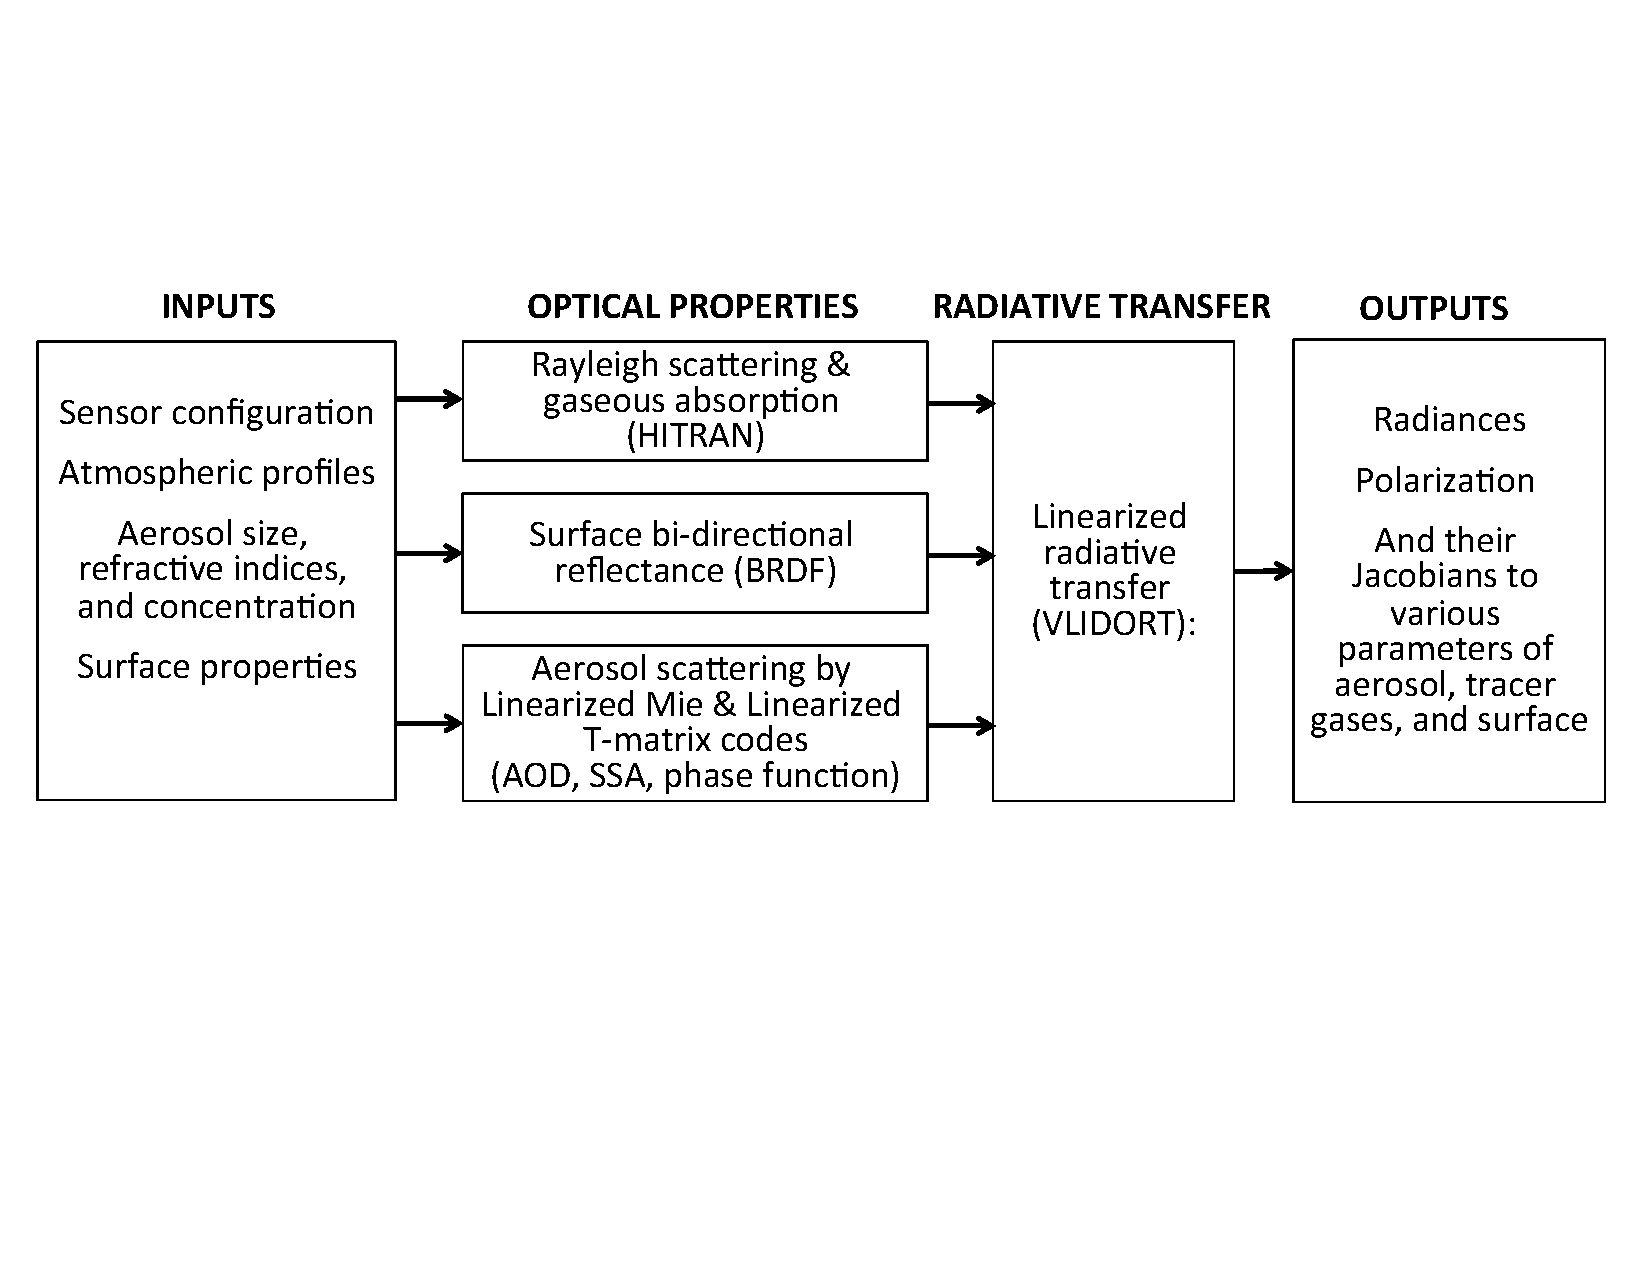
\includegraphics[width={0.95\textwidth}]{figures/unlvrtm.pdf}
  \caption{Flowchart of the UNL-VRTM components. See text for detail.}
  \label{fig:unlvrtm}
\end{figure}

Inputs for the UNL-VRTM are profiles of atmospheric properties and
constituents (temperature, pressure, aerosol mass concentration or layer
AOD, water vapor amount and other trace gas volume mixing ratio
profiles \citep{McClatchey72}), the surface properties, as well as 
the aerosol parameters  (such as PSD parameters and refractive index)
themselves. Bearing in mind the lack of
sensitivity in passive remote sensing for the retrieval of vertical
profiles of aerosol properties, the UNL-VRTM as it stands now is only
designed to deliver radiative calculations for a maximum of two sets of
aerosol single scattering properties (e.g., aerosol PSD,
refractive index, and particle shape), typically with one fine-mode and
one coarse-mode aerosol. Other inputs for model include spectral and
geometrical definitions that characterizing specification of an
observing sensor. 

Outputs of the model include the Stokes vector ($\mathbf{I}$) at
user-defined spectral wavelengths and desired atmospheric
levels for both upwelling and downwelling radiation, from which the
light radiance and degree of polarization can be derived. Outputs also
include analytical Jacobians of $\mathbf{I}$ with respect to all aerosol
particle parameters (PSD, refractive index, vertical profile), Rayleigh
scattering optical depth, optical depth of all trace gases, and
parameters describing surface optical property. A detail description of
the UNL-VRTM's Jacobian capability is presented in section
\ref{subsec:jacobian}. 

Although the UNL-VRTM is used to simulate the AERONET measurements in
this work, the module-based sturcture of UNL-VRTM allows its application 
not limit to the AERONET inversion. 
It can be easily used to simulate observations
from other remote sensing platforms, like satellite sensors. For
example, we have employed it to explore the aerosol information content
of observations from the future TEMPO/GEO-CAPE geostationary satellite
sensors \citep{Wang14}, to investigate the potential application of
hyperspectral radiances at \ce{O2}A and \ce{O2}B bands for retrieving
aerosol vertical profile \citep{Wang14, Ding14}, to retrieve aerosol 
microphysical properties from GeoTASO measured UV-to-visible contiuneous 
radiance spectra \citep{Hou14}, and to perform AOD retrieval from 
GOSAT/TANSO-CAI's UV radiance \citep{Han14}. 

Recently, we have made the UNL-VRTM publicly accessible. We published
the source code on \url{http://meteo.unl.edu/~xxu/unlvrtm.php}. A
detail description and a dedicated User's Guide for the model is also 
available on the webpage.  

\subsection{Molecular scattering and absorption} \label{subsec:rayleigh}

The Rayleigh scattering optical depth at certain wavelength in any 
atmospheric layer ($\taur$) is computed by
\begin{equation}
\taur = N_\text{air}\sigma_\text{R} 
\end{equation}
where $N_\text{air}$ is air molecular number density of that layer
(molec cm$^{-2}$), and $\sigma_\text{R}$ is the Rayleigh scattering 
cross-section (cm$^2$ molec$^{-1}$) computed following
\citet{Bodhaine99}. The Rayleigh phase matrix,
$\mathbf{P}_\text{R}(\Theta)$, depends upon molecular 
anisotropy through the depolarization factor, also computed from the same 
source. \citet{Bodhaine99} computes the wavelength-dependent Rayleigh
scattering cross-section as a function of mixing ratios for \ce{N2},
\ce{O2}, \ce{H2O}, and \ce{CO2}. The phase matrix for Rayleigh scattering
follows \citet{Hansen74}; we use the set of spherical-function expansion
 coefficients for the phase matrix as supplied for VLIDORT
\citep{Spurr06}.

Calculation of the absorption optical depth ($\taug$) at
any atmospheric layer for $K$ different trace gases follows
\begin{equation}
\taug = \sum_{i=1}^K N_{\text{gas,}i}\sigma_{\text{A,}i}(T,P) 
\end{equation}
where $N_{\text{gas,}i}$ is the number density of \textit{i}th gas
within that layer, and $\sigma_{\text{A,}i}$ is the corresponding
absorption cross-section, a function of temperature and pressure. 
Our model accounts for absorptions by a total number of
22 trace gases: \ce{H2O}, \ce{CO2}, \ce{O3}, \ce{N2O}, \ce{CO},
\ce{CH4}, \ce{O2}, \ce{NO}, \ce{SO2}, \ce{NO2}, \ce{NH3}, \ce{HNO3},
\ce{OH}, \ce{HF}, \ce{KCl}, \ce{HBr}, \ce{HI}, \ce{ClO}, \ce{OCS},
\ce{H2CO}, \ce{HOCl}, and \ce{N2}.
The determination of $\sigma_\text{A}$  
utilizes a UV-to-visible cross-section library and the line-spectroscopic
absorption parameters archived in the HITRAN database \citep{Orphal03,
Rothman09}. The cross-section library compiles the extinction
cross-section for \ce{O3}, \ce{NO2}, \ce{SO2}, and \ce{O2-O2} in the UV
and/or visible spectral regions. Meanwhile, line-spectroscopic 
absorption databased are used to simulate the pressure- and
temperature-dependent extinction cross-section with line-by-line (LBL) 
approach \citep{Liou02,Rothman09} by accumulating each individual 
absorption line. Doppler broadening is calculated from the molecular mass
and the temperature, and Doppler and Lorentz broadening are included in the
Voigt calculation.

Particular to work, we only consider the most influential 
trace species for the AERONET spectral bands: \ce{H2O} (vapor), \ce{O3}, 
and \ce{NO2}. In our algorithm (section \ref{ch:algorithm}), the columnar
amounts of \ce{O3} and \ce{NO2} are dynamically adjusted with retrievals from the
Ozone Monitoring Instrument (OMI) \citep{Levelt06} on board the
AURA satellite. We apply the columnar water vapor amount retrieved from
the 940-nm radiances measured by the AERONET SunPhotometer
\cite{Halthore97}.

\subsection{Aerosol single scattering} \label{subsec:mie}

Aerosol single scattering properties necessary to the radiative
transfer calculation include aerosol optical depth ($\taua$)
($\qext$), SSA ($\assa$), and scattering phase matrix ($\paer(\Theta)$).
The calculation of these parameters is made with a Linearized Mie (LMIE)
scattering electromagnetic code for spherical particles and a Linearized
T-matrix (LTMATRIX) scattering code for non-spherical convex and axially
symmetric particles \citep{Spurr12}. The LMIE code originates from the Mie code
of \citet{deRooij84}, and the LTMATRIX code originates from the T-Matrix
code developed by \citet{Mishchenko96, Mishchenko98}; both include
linearization capabaility developed by \citet{Spurr12}.

Common inputs for both codes are the complex refractive index
($\mreal + i\mimag$), and the particle size distribution (PSD) 
parameters for polydisperse scattering. The codes have several options 
to specify the PSD function: two-parameter gamma, two-parameter 
lognormal, three-parameter modified gamma, and four-parameter bi-lognormal. 
In addition, the linearized T-matrix code offers options to characterize the 
shape of non-spherical aerosols (spheroids, cylinders, or Chebyshev particles)
\citep{Spurr12}. For non-spherical particles, the specified size distribution 
is interpreted as the equivalent surface-area sphere in the linearized T-matrix
calculation, regardless of the shape. 

For AERONET inversion alorithm, we assume that the aerosol volume
distribution follows a bi-modal lognormal function \citep[in agreement
wit][]{Schuster06, Waquet09}:
\begin{equation}
\frac{\text{d}V}{\text{d}\ln{r}} = \sum_{i=1}^2 
\frac{V_0^i}{\sqrt{2\pi}\ln{\sg^i}} 
\exp{\left[ -\frac{(\ln{r}-\ln{\rv^i})^2}{2\ln^2{\sg^i}}\right]}
\label{eq:bilognormal}
\end{equation}
where $V_0$, $\rv$, and $\sg$ are the total volume concentration, geometric
median radius, and standard deviation, respectively. The superscript $i$
indicates the size mode, and later will be replaced by ‘f’ for fine mode
and ‘c’ for coarse mode. We assume that particle size ranges from 0.01
to 10 $\mu$m for the fine mode and from 0.05 to 20 $\mu$m for
the coarse mode, both covering $>$ 99.9\% of the total volume of an 
idealistic size range (0, $+\infty$). An advantage of the lognormal 
distribution is that standard deviations for the number, area, and 
volume PSD functions are identical, and therefore allowing that the 
median radii for these PSD functions can be converted from one to 
another \citep{Seinfeld06}. The $\reff$ and $\veff$ are related to 
the geometric parameters through:
\begin{align}
\reff &= \rv \exp{\left( -\frac{1}{2} \ln^2{\sg}\right)}, \\
\veff & = \exp{\left(\ln^2{\sg}\right)} - 1.
\end{align}

The LMIE/LTMATRIX code computes the aerosol extinction efficiency
factor $\qext$, single scattering albedo $\assa$, and phase matrix 
$\paer(\Theta)$, as well as Jacobians of these quantities with respect
to input parameters including $\reff$, $\veff$, $\mreal$, and $\mimag$.
The phase matrix and its Jacobians are expressed in terms of the
coefficients $\baer(\Theta)$ for each moment $l$ in terms of the 
generalized spherical function expansions
for each non-zero phase matrix element. Let $\mathbf{A}$ denotes the
vector of aerosol microphysical parameters, 
$\mathbf{A}=[V_0,\reff,\veff,\mreal,\mimag]^T$, and $\mathbf{M}$
the vector of aerosol optical parameters, 
$\mathbf{M}=[\taua,\assa,\baer(\Theta)]^T$, 
where $\taua$ is related to $\qext$ by 
$\taua=\frac{3V_0 \qext}{4\reff}$. The LMIE/LTMATRIX code acts
as an operator that maps vector $\mathbf{A}$ to $\mathbf{M}$. 
The Jacobian matrix of $\mathbf{M}$ with respect to $\mathbf{A}$ calculated by 
means of the linearization feature of the code, and it can be expressed by
$\nabla_\mathbf{A}\mathbf{M}$. 

\subsection{Surface representations} \label{subsec:surface}

VLIDORT has a supplementary module for specification of the surface BRDF
as a linear combination of (up to) three semi-empirical kernel
functions; for details, see \citet{Spurr04}. This supplementary module can also
provide partial derivatives of the BRDF with respect to the kernel
weighting factors or with respect to kernel parameters such as the wind
speed for glitter reflectance. These kernel functions include
Lambertian, Ross-Thick, and Li-Sparse functions \citep{Wanner95, Lucht00}, a
Bi-directional Polarization Distribution Function (BPDF)
\citep{Maignan09}, and an ocean surface model based on the 
Cox-Munk model \citep{Cox54}. In addition, VLIDORT has
an option for using a surface-leaving radiation field, either as a
fluorescence term or as a water-leaving term expressed as a function of
chlorophyll absorption.

Although surface reflectance has in general a low influence on AERONET
down-welling sky radiances and polarization, a state-of-the-art
representation of the surface reflectivity potentially reduces model
uncertainties, especially for measurements taken at low elevation angles
that could be affected by surface diffusion. Here, we utilize the
spectral BRDF parameters from the MODIS surface products that are
operationally reported every 16 days at a 1-km resolution
\citep{Lucht00}. Here we use time-matched MODIS BRDF products 
to reconstruct the bidirectional reflectance over AERONET stations.
The MODIS BRDF product supplies three weighting parameters
($f_\text{iso}$, $f_\text{vol}$, and $f_\text{geo}$) for the first 
7 MODIS bands, respectively, corresponding to three kernel types:
isotropic, Ross-Thick ($K_\text{vol}$), and Li-Sparse ($K_\text{geo}$):
\begin{equation}
\rho_\text{R}(\mu,\phi;\mu_0,\phi_0) = f_\text{iso} + 
f_\text{vol}K_\text{vol}(\mu,\phi;\mu_0,\phi_0) +
f_\text{geo}K_\text{geo}(\mu,\phi;\mu_0,\phi_0)  \label{eq:brdf}
\end{equation}
Expanded expressions for $K_\text{vol}$ and $K_\text{geo}$ appear in
\citet{Wanner95, Lucht00}. 

Studies have shown that the BPDF for land surfaces is generally rather
small and is “spectrally neutral” \citep{Nadal99, Maignan04, Maignan09,
Waquet07, Litvinov11}. 
Most empirical BPDF models are based on Fresnel coefficients of light
reflectance from the surface. Here we have incorporated the
one-parameter model developed by \citet{Maignan09}, which was
derived from analyses of several years of POLDER/PARASOL measurements.
This model describes the polarized reflectance at any viewing geometry
($\mu$, $\phi$) from the given incident geometry ($\mu_0$, $\phi_0$) as:
\begin{equation}
\pmb{\rho}_\text{P}(\mu,\phi;\mu_0,\phi_0) = 
\frac{C_0 \exp(-\tan \theta_\text{h})\exp(-\text{NDVI})}{\mu_0+\mu} 
\mathbf{F}_\text{P}(\theta_\text{h},n_\text{v}) \label{eq:bpdf}
\end{equation}
where $C_0$ is a constant parameter chosen for a certain surface type,
$\theta_\text{h}$ is half of the phase angle of reflectance, $n_\text{v}$ is 
the refractive index of vegetation (1.5 is used), and
$\mathbf{F}_\text{P}$ is the Fresnel reflection matrix. 
We chose a spectrally-independent value for $C_0$ based
on the recommendations by \citet{Maignan09} for relevant surface types. 

The combination of the BRDF and BPDF for land surface follows the
discussion by \citet{Dubovik11}. The surface reflectance matrix 
$\mathbf{R}_\text{s}(\mu,\phi;\mu_0,\phi_0)$
is represented as a sum of diffuse unpolarized
reflectance and specular reflectance; the former is modeled using the
MODIS BRDF in equation \eqref{eq:brdf}, and the latter using the BPDF 
formula in equation \eqref{eq:bpdf}. 

\subsection{Radiative transfer} \label{subsec:vlidort}

The radiative transfer equation \eqref{eq:rte} is solved with the 
Vector Linearized Discrete Ordinate Radiative Transfer (VLIDORT)
model, which is a core part of the UNL-VRTM. VLIDORT, 
developed by \citet{Spurr06}, is a
linearized pseudo-spherical vector discrete ordinate radiative transfer
model for multiple scattering of diffuse radiation in a stratified
multi-layer atmosphere. It computes four elements of the Stokes vector I
for downwelling and upwelling radiation at any desired atmospheric
level. The VLIDORT includes the pseudo-spherical approximation to
calculate solar beam attenuation in a curved medium. It also uses the
delta-M approximation for dealing with sharply peaked forward
scattering. Specifically for the AERONET inversion, we consider 16
discrete ordinate streams in the radiative transfer calculation and
retain 180 terms in the spherical-function expansion of the scattering
matrix to ensure accurate calculation of diffuse radiation. 

Along with the Stokes vector $\mathbf{I}$, VLIDORT also computes the Jacobian
matrix of I with respect to aerosol optical vector $\mathbf{M}$, 
$\nabla_\mathbf{M}\mathbf{I}$. Therefore,
the combination of the VLIDORT and the LMIE/LTMATRIX codes allows for a
direct calculation of the Jacobian matrix of the Stokes vector with
respect to aerosol microphysics, $\mathbf{A}$, by
\begin{equation}
\nabla_\mathbf{A}\mathbf{I} = \nabla_\mathbf{M}\mathbf{I}
\cdot \nabla_\mathbf{A}\mathbf{M} \label{eq:adj-i}
\end{equation}
Essentially, the above equation can yield the derivatives of the
radiance $I$ and $\dolp$ with respect to any aerosol microphysical parameter,
i.e., $\nabla_\mathbf{A}I$ and $\nabla_\mathbf{A}\dolp$. 
While obtaining $\nabla_\mathbf{A}I$ is straightforward,
$\nabla_\mathbf{A}\dolp$ can be derived from equation \eqref{eq:dolp} 
following:
\begin{equation}
\nabla_\mathbf{A}\dolp = -\frac{\dolp \nabla_\mathbf{A}}{I} +
\frac{Q\nabla_\mathbf{A}{Q}+U\nabla_\mathbf{A}{U}}{I\sqrt{Q^2+U^2}}
\label{eq:adj-dolp}
\end{equation}

\subsection{Capability of calculating Jacobians} \label{subsec:jacobian}

This section analytically derives the Jacobian of $\mathbf{I}$ with
respect to various aerosol related parameters, including $\taua$,
$\assa$, $\baer$, refractive index, PSD parameters, and aerosol vertical
profile. Computation of the Stokes vector in VLIDORT requires input of
an optical property set $[\tau,\omega,\left<\mathbf{B}^j\right>_{j=0,J}]$ for
each atmospheric layer, where $<>_{j=0,J}$ denotes the vector that
consists of elements having the similar expression as that inside $<>$
but for $j=0, J$. For each atmospheric layer $L$, the optical property
inputs are assumed constant and are given by equations 
\eqref{eq:opt1}--\eqref{eq:opt2}, as well as equation \eqref{eq:opt3}
with $\mathbf{P}(\Theta)$ replaced by $\mathbf{B}^j$. 
It should be noted that all parameters
in these requations are for each layer, but we ignore $L$ for
convenience.

Since VLIDORT generates Jacobians with respect to layer-integrated
single scattering properties in each atmospheric layer as well as
column-integrated single scattering property as a whole, and LMIE and
LTMATRIX offer the sensitivity of aerosol scattering properties to
microphysical aerosol physical parameters, an integrated use of VLIDORT
and LTMATRIX/LMIE can, in principle, provide the Jacobians of Stokes
parameters with respect to both aerosol single scattering properties as
well as aerosol microphysical parameters (as expressed by equations
\eqref{eq:adj-i}--\eqref{eq:adj-dolp}). Practically, the VLIDORT
calculation of Jacobians of any Stokes parameter $\xi$ with respect to 
any aerosol parameter $x$ proceeds according to
\begin{equation}
\begin{split}
x\frac{\ptxi}{\partial x} &=
  x\left[ \frac{\ptxi}{\pttau}, \frac{\ptxi}{\ptssa}, 
          \left< \frac{\ptxi}{\ptb^j}\right>_{j=1,J}\right] 
  \left[ \frac{\pttau}{\ptx}, \frac{\ptssa}{\ptx}, 
         \left< \frac{\ptb^j}{\ptx}\right>_{j=1,J}\right]^T \\
  &= \left[ \tau \frac{\ptxi}{\pttau}, \omega \frac{\ptxi}{\ptssa}, 
          \left< \mathbf{B}^j \frac{\ptxi}{\ptb^j}\right>_{j=1,J}\right]
     \left[ \phi_x, \varphi_x, \left< \pmb{\Psi}_x^j\right>_{j=1,J}
\right]^T. 
\end{split}
\label{eq:adj-x}
\end{equation}

The first square bracket on the right-hand side of equation
\eqref{eq:adj-x} contains quantities computed internally by VLIDORT, 
while the second so-called “transformation vector” must be supplied 
by users and is defined as:
\begin{equation}
\phi_x = \frac{x}{\tau}\frac{\pttau}{\ptx}; \quad 
\varphi_x = \frac{x}{\omega}\frac{\ptssa}{\ptx}; \quad 
\pmb{\Psi}_x^j = \frac{x}{\mathbf{B}^j}\frac{\ptb^j}{\ptx}.
\label{eq:lopt}
\end{equation}

%% Table 
\begin{table}[t]
  \centering
  \small
  \caption{Elements of transformation vector for various aerosol single
scattering parameters (composite of fine and coarse mode).}
  \label{tab:jacobian1}
  \begin{tabular}{p{2em} p{2em} p{5em} p{15em} }
    \toprule
       $x$ & $\phi_x$ & $ \varphi_x$ & $\pmb{\Psi}_x^j$ \\
    \midrule
    $\taua$        & $\frac{\taua}{\tau}$ &
$\frac{\taua}{\tau}\left( \frac{\assa}{\omega}-1\right)$ &
$\left\{ \begin{array}{ll} \frac{\assa\taua}{\omega\tau}\left(
\frac{\baer^j}{\mathbf{B}^j}-1 \right)
&\mbox{for } j<3  \\ \frac{\taur}{\omega\tau} & \mbox{for } j\geq 3
\end{array} \right.$\\  
    $\assa$        & 0 & $\frac{\taua\assa}{\tau\taua\assa+\taur}$ &
Same as above \\
    $B_\text{A}^j$ & 0 & 0 & $\left\{ \begin{array}{ll}
\frac{\assa\taua\baer^j}{\assa\taua\baer^j+\taur\mathbf{B}_\text{R}^j}
&\mbox{for } m=j<3  \\ 1 & \mbox{for } m=j\geq 3 \\ 0 & \mbox{for }
m\neq j
\end{array} \right.$ \\
    \bottomrule
  \end{tabular}
\end{table}

As we are interested in aerosol parameters, this transformation vector
can be further expanded as 
\begin{equation}
\left[ \phi_x, \varphi_x, \left< \pmb{\Psi}_x^j\right>_{j=1,J}\right]^T
=\pmb{\Pi} \left[ \phi_x^\prime, \varphi_x^\prime, \left<
\pmb{\Psi}_x^{\prime j}\right>_{j=1,J}\right]^T, \label{eq:trans}
\end{equation}
where
\begin{equation}
\phi_x^\prime = x\frac{\pttaua}{\ptx}, \quad 
\varphi_x^\prime = x\frac{\ptscaa}{\ptx}, \quad  \mbox{and} 
\pmb{\Psi}_x^{\prime j} = x\frac{\ptbaer^j}{\ptx},
\label{eq:alopt}
\end{equation}
and $\pmb{\Pi}$ is a matrix expressed by
\begin{equation}
\pmb{\Pi} = \left[ 
            \begin{array}{lll}
            \frac{1}{\tau}  & \pmb{0} & \pmb{0} \\
            -\frac{1}{\tau} & \frac{1}{\scaa+\taur} & \pmb{0} \\
            \pmb{0} & \left<
\frac{\baer^j-\bray^j}{\mathbf{B}^j(\scaa+\taur)}\right>_{j=1,J} & 
\left< \frac{\scaa}{\mathbf{B}^j(\scaa+\taur)}\right>_{j=1,J}
            \end{array}
            \right]. \label{eq:pi}
\end{equation}
Here, $\scaa$ is the scattering optical depth of aerosols. The detailed
derivations of the matrix $\pmb{\Pi}$ are presented in Appendix \ref{app:pi}. 
Hence, the transformation vector for calculating Stokes profile Jacobians 
with respect to $\taua$, $\assa$, $\baer^j$ can be obtained by combining 
equations \eqref{eq:trans} and \eqref{eq:pi}, and the components of 
this vector are listed in Table \ref{tab:jacobian1}.

In an atmosphere where both fine (superscript “f”) and coarse
(superscript “c”) aerosol particles co-exist, the ensemble aerosol
optical properties may be derived by assuming external mixing:
\begin{equation}
\left\{  
\begin{array}{ll}
\taua &= \taua^\text{f} + \taua^\text{c} \\
\scaa &= \scaa^\text{f} + \scaa^\text{c} \\
\baer^j &= \frac{\scaa^\text{f} + \scaa^\text{c}}
           {\scaa^\text{f}\baer^{\text{f},j} + \scaa^\text{c}\baer^{\text{c},j} }
\end{array} 
\right.
\end{equation}


\begin{table}[t]
  \centering
  \small
  \caption{Elements of transformation vector for various microphysical
parameters of fine and coarse mode aerosols\textsuperscript{a}.}
  \label{tab:jacobian2}
  \begin{tabular}{p{4em} p{10em} p{10em} p{11em} }
    \toprule
       $x$ & $\phi_{x\fine}^\prime$ & $\varphi_{x\fine}^\prime$ &
$\pmb{\Psi}_{x\fine}^{\prime j}$ \\
    \midrule
    $\taua\fine$ & $\taua\fine$ & $\scaa\fine$ & 
    $\frac{\scaa\fine}{\taua}(\baer^{\text{f}j}-\baer^j)$ \\
    $\assa$ & 0 & $\scaa\fine$ &
    $\frac{\scaa\fine}{\taua}(\baer^{\text{f}j}-\baer^j)$ \\ 
    $V_0\fine$ & $\frac{3V_0\fine\qext\fine}{4\reff\fine}$ &
    $\frac{3V_0\fine\qsca\fine}{4\reff\fine}$ &
    $\frac{\scaa\fine}{\taua}(\baer^{\text{f}j}-\baer^j)$ \\ 
    $\mreal\fine,\mimag\fine$ & 
    $\taua\fine\frac{x\fine}{\qext\fine}\frac{\partial\qext\fine}{\ptx\fine}$ &
    $\scaa\fine\frac{x\fine}{\qsca\fine}\frac{\partial\qsca\fine}{\ptx\fine}$ & 
    $\frac{\varphi_{x\fine}^\prime}{\scaa\fine}(\baer^{\text{f}j}-\baer^j)+x\fine\frac{\partial\baer^{\text{f}j}}{\ptx\fine}$ \\
    $\rg\fine,\sg\fine,\epsilon\fine$ &
    $\taua\fine(\frac{x\fine}{\qext\fine}\frac{\partial\qext\fine}{\ptx\fine}-\frac{x\fine}{\reff\fine}\frac{\partial\reff\fine}{\ptx\fine})$ & 
    $\scaa\fine(\frac{x\fine}{\qsca\fine}\frac{\partial\qsca\fine}{\ptx\fine}-\frac{x\fine}{\reff\fine}\frac{\partial\reff\fine}{\ptx\fine})$ &
    $\frac{\varphi_{x\fine}^\prime}{\scaa\fine}(\baer^{\text{f}j}-\baer^j)+x\fine\frac{\partial\baer^{\text{f}j}}{\ptx\fine}$ \\
    $H\fine$ & $H\fine\frac{\pttaua}{\partial{H\fine}}$ &
    $\phi_{x\fine}^\prime\assa\fine$ &
    $\frac{\scaa\fine}{\taua}(\baer^{\text{f}j}-\baer^j)$ \\
    \bottomrule
    \multicolumn{4}{m{35em}}{\textsuperscript{a}
Expressions are shown only for fine-mode parameters; expressions for
coarse-mode parameters are the same but with superscripts replaced by
'c'}
  \end{tabular}
\end{table}

We can generate the transformation vectors (as listed in Table
\ref{tab:jacobian2}) for any of the following parameters: $\taua\fine$, 
$\assa\fine$, $V_0\fine$, $\mreal\fine$, $\mimag\fine$, $\rg\fine$,
$\sg\fine$, $\epsilon\fine$, $H\fine$, and $\taua\coarse$,
$\assa\coarse$, $V_0\coarse$, $\mreal\coarse$, $\mimag\coarse$,
$\rg\coarse$, $\sg\coarse$, $\epsilon\coarse$, and $H\coarse$. Here,
$\rg$, $\sg$, and $H$ denote the median and standard deviation of the
particle radius (e.g., two parameters in the log-normal aerosol number
distribution), and the scale height of aerosol extinction, respectively.
$V_0$ is the aerosol volume concentration and $\epsilon$ the shape 
factor of the non-spherical particle. Details of the algebra for deriving 
the transformation vectors may be found in Appendix \ref{app:pi}. 
Note that the shape of the aerosol extinction vertical profile in the
testbed is assumed to be constant or exponentially decreasing with
height or quasi-Gaussian (Appendix \ref{app:pi}). The analytical
formulas for $\phi_x^\prime$, $\varphi_x^\prime$, and
$\pmb{\Psi}_x^{\prime j}$ for coarse mode aerosol parameters are
the same as their counterparts for fine-mode aerosols; we need only
replace superscript “s” with “c” in Table 3 entries. Jacobians with
respect to the fine mode fraction, either in terms of AOD
($\fmftau$) or in terms of the volume concentration ($\fmfv$), 
can be derived from the corresponding Jacobians with respect to 
modal AOD and volume, respectively:
\begin{align}
\fmftau\frac{\ptxi}{\partial\fmftau} & = 
   \taua\fine\frac{\ptxi}{\partial\taua\fine} - 
   \frac{\fmftau}{1-\fmftau}\taua\coarse\frac{\ptxi}{\partial\taua\coarse} \\
\fmfv\frac{\ptxi}{\partial\fmfv} & = 
   V_0\fine\frac{\ptxi}{\partial{V_0}\fine} - 
   \frac{\fmfv}{1-\fmfv}V_0\coarse\frac{\ptxi}{\partial{V_0}\coarse}
\end{align}

Details of these necessary VLIDORT inputs are presented in Appendix
\ref{app:pi}, and a comprehensive verification of these Jacobian calculation are
presnted in following section {\ref{sec:rtmverify}}.

%%%% New section
\section{Model Benchmarking and Verifications} \label{sec:rtmverify}

\begin{figure}[p]
  \centering
  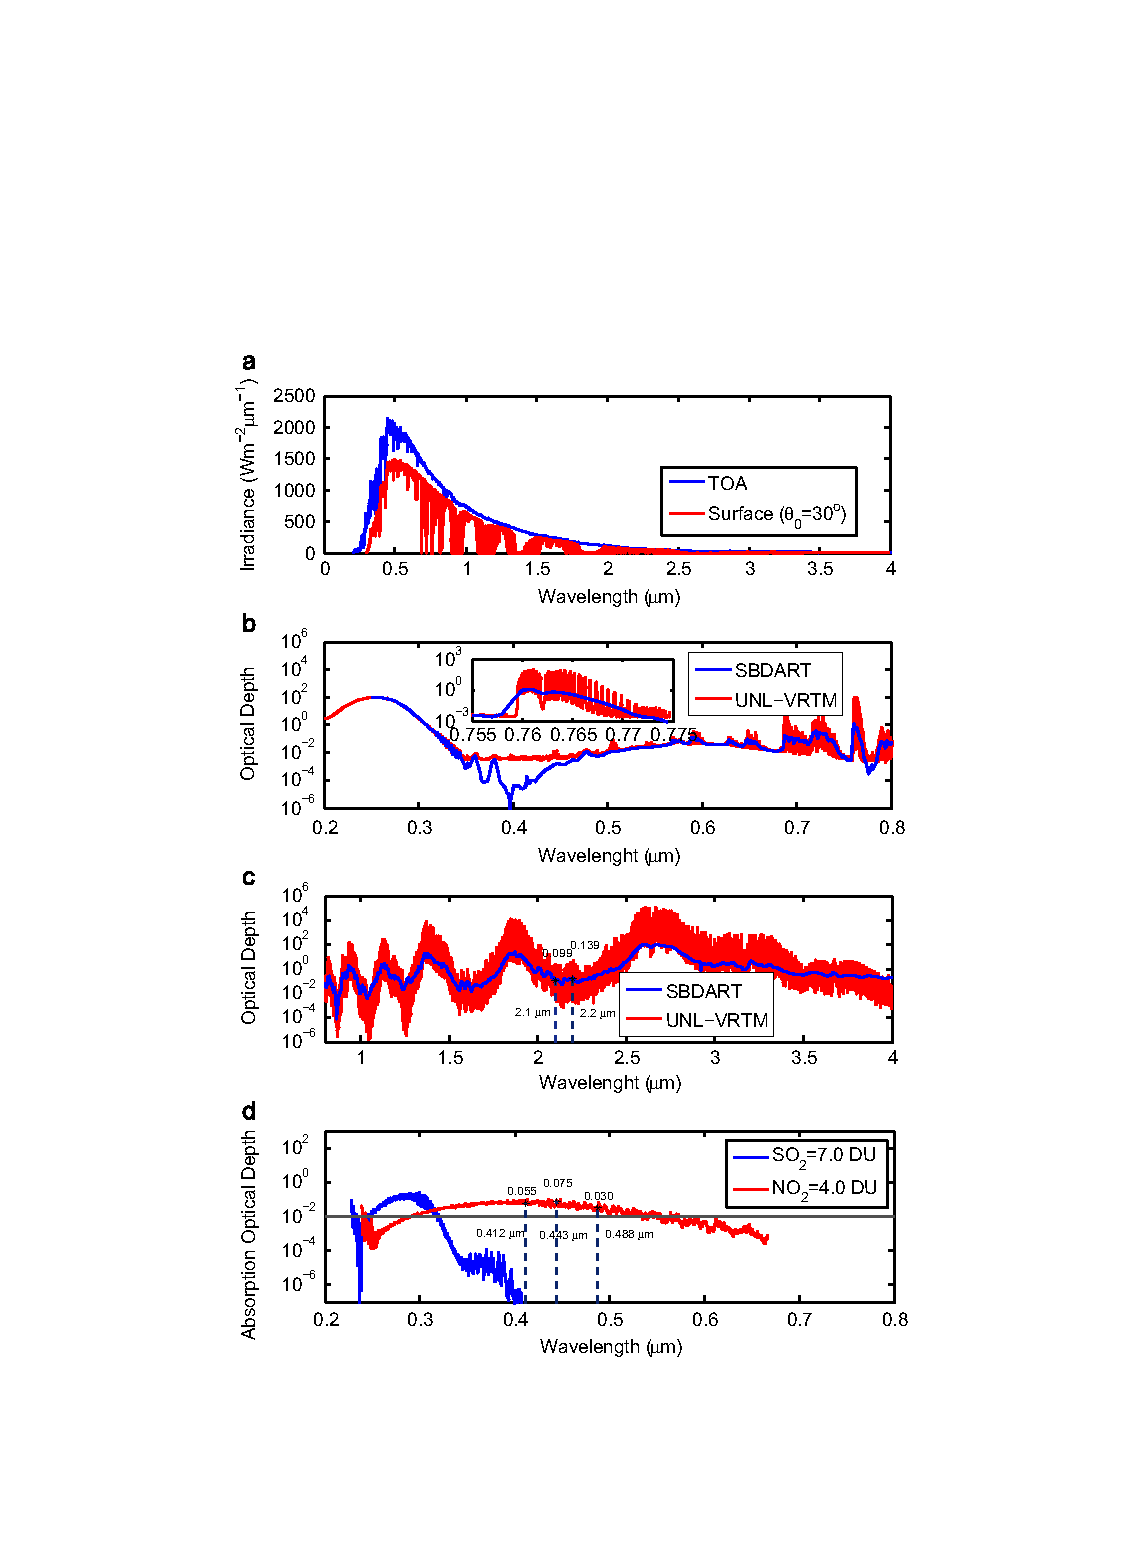
\includegraphics[width={0.8\textwidth}]{figures/unlvrtm1.pdf}
  \caption{Some benchmark simulations by the UNL-VRTM: 
(a) Downward solar spectral irradiance at the TOA and the
surface for solar zenith angle of 30$^\circ$. (b) Total-atmosphere gas
absorption optical depth in the range 0.2--0.8 $\mu$m. (c) Same as (b) but
for 0.8--4 $\mu$m. (d) Optical depth of \ce{SO2} and \ce{NO2} in
 polluted cases. Also shown in (b) and (c) are the optical depth computed 
from Santa Barbara DISORT Atmospheric Radiative Transfer (SBDART) model
\citep{Ricchiazzi98}. The mid-latitude summer atmospheric profile is 
assumed \citep{McClatchey72}. (Figure adopted from \citet{Wang14}.)}
  \label{fig:unlvrtm1}
\end{figure}

Figure \ref{fig:unlvrtm1}a shows the downward solar spectral irradiance 
at the top-of-atmosphere and at the surface for a solar zenith angle of
30$^\circ$. Spectral regions dominated by gas absorption can be 
clearly identified, including the \ce{O3} Hartley-Huggins bands 
in the UV, the \ce{O2}B band (0.69 $\mu$m) and \ce{O2}A band (0.76 
$\mu$m), as well as a number of water vapor bands. The
spectroscopic calculations shown in Figure \ref{fig:unlvrtm1} were 
performed at a resolution of 0.01 nm. In general this resolution is 
high enough to pick up fine structure in gas absorptions. 
In the UV below 300 nm, and in parts of the \ce{O2}A and \ce{O2}B 
bands, whole-atmosphere gas absorption optical depths can reach 
50 or more, and the downward irradiance is nearly zero
at the ground (Figure \ref{fig:unlvrtm1}b). The inset in Figure
\ref{fig:unlvrtm1}b shows a close-up view of the fine structure 
in absorption optical depth for the \ce{O2}A band, with
dual peaks centered at 0.761 $\mu$m and 0.764 $\mu$m, and a deep, 
narrow valley around 0.762 $\mu$m. Similarly, the continuum of water 
vapor absorption from the near-infrared to about 4 $\mu$m is also well 
simulated (Figure \ref{fig:unlvrtm1}c). Also of note is the 
non-negligible absorption of \ce{SO2} and \ce{NO2} in UV and blue
wavelength regions respectively (Figure \ref{fig:unlvrtm1}d). 
In urban regions, high \ce{SO2} and \ce{NO2} can together contribute 
optical depths of around 0.03--0.07 (Figure \ref{fig:unlvrtm1}d). 
Hence, in order to take advantage of low surface reflectance
in the UV and the use of deep-blue wavelengths for the retrieval of AOD
in urban regions, it is critical to treat absorption by \ce{SO2} and
\ce{NO2}. In contrast, calculations performed at moderate spectral 
resolution (such as those from Santa Barbara Discrete-Ordinate Atmospheric 
Radiative Transfer, or SBDART \citep{Ricchiazzi98}, shown as the blue 
lines in Figure \ref{fig:unlvrtm1}b and c) do not resolve fine-structure 
details, sometimes missing the absorption lines for \ce{SO2} or \ce{NO2}, 
and in general producing significant underestimation of optical depths 
in the \ce{O2}A band.

\begin{figure}[t]
  \centering
  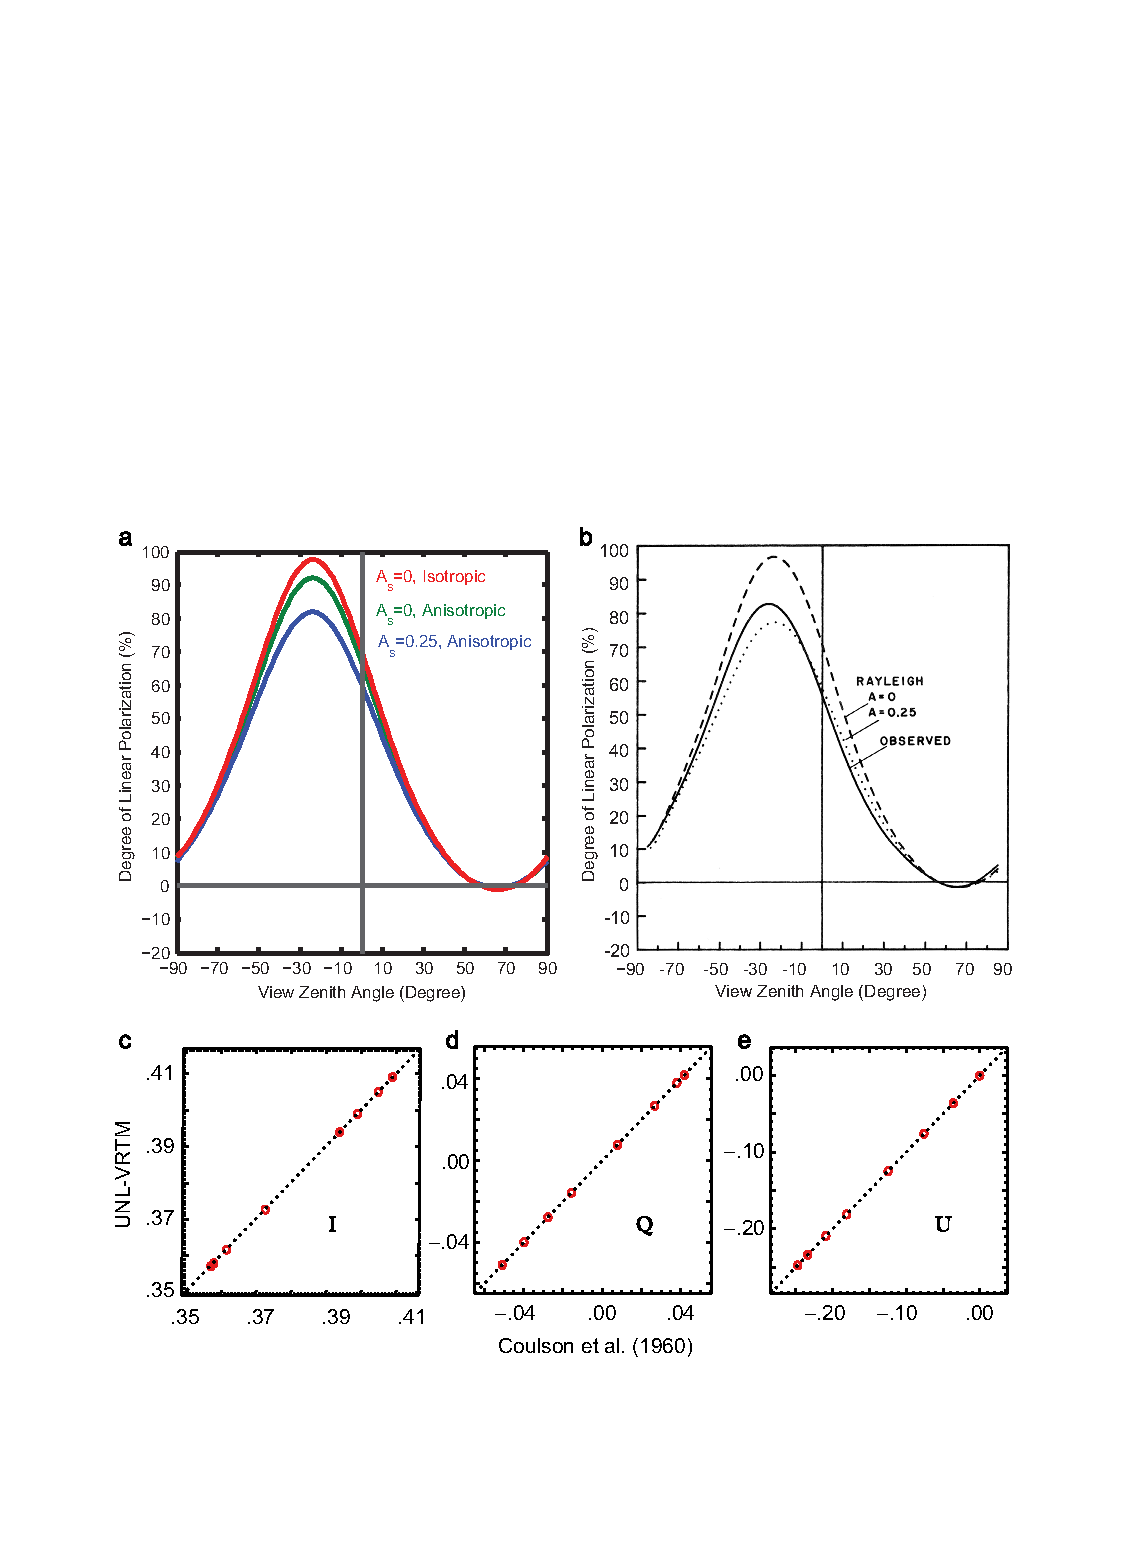
\includegraphics[width={0.8\textwidth}]{figures/unlvrtm2.pdf}
  \caption{Degree of linear polarization ($-Q/I$) of downward radiation
for a pure Rayleigh atmosphere: (a) computed by UNL-VRTM for the case
analyzed in Figure 5.7 of \citet{Coulson88} and shown here as (b). (c)--(e)
shows the comparisons of $I$, $Q$, and $U$ computed by \citet{Coulson60} and
those from UNL-VRTM. In (a) and (b), $A_\text{s}$ represents the surface albedo
value. In (c) and (d), the calculation is for $\tau=1.0$, surface albedo
is 0.25, $\cos{\theta_0}=0.8$, and for 8 different viewing angles.
(Figure adopted from \citet{Wang14}.)}
  \label{fig:unlvrtm2}
\end{figure}

\begin{figure}[t]
  \centering
  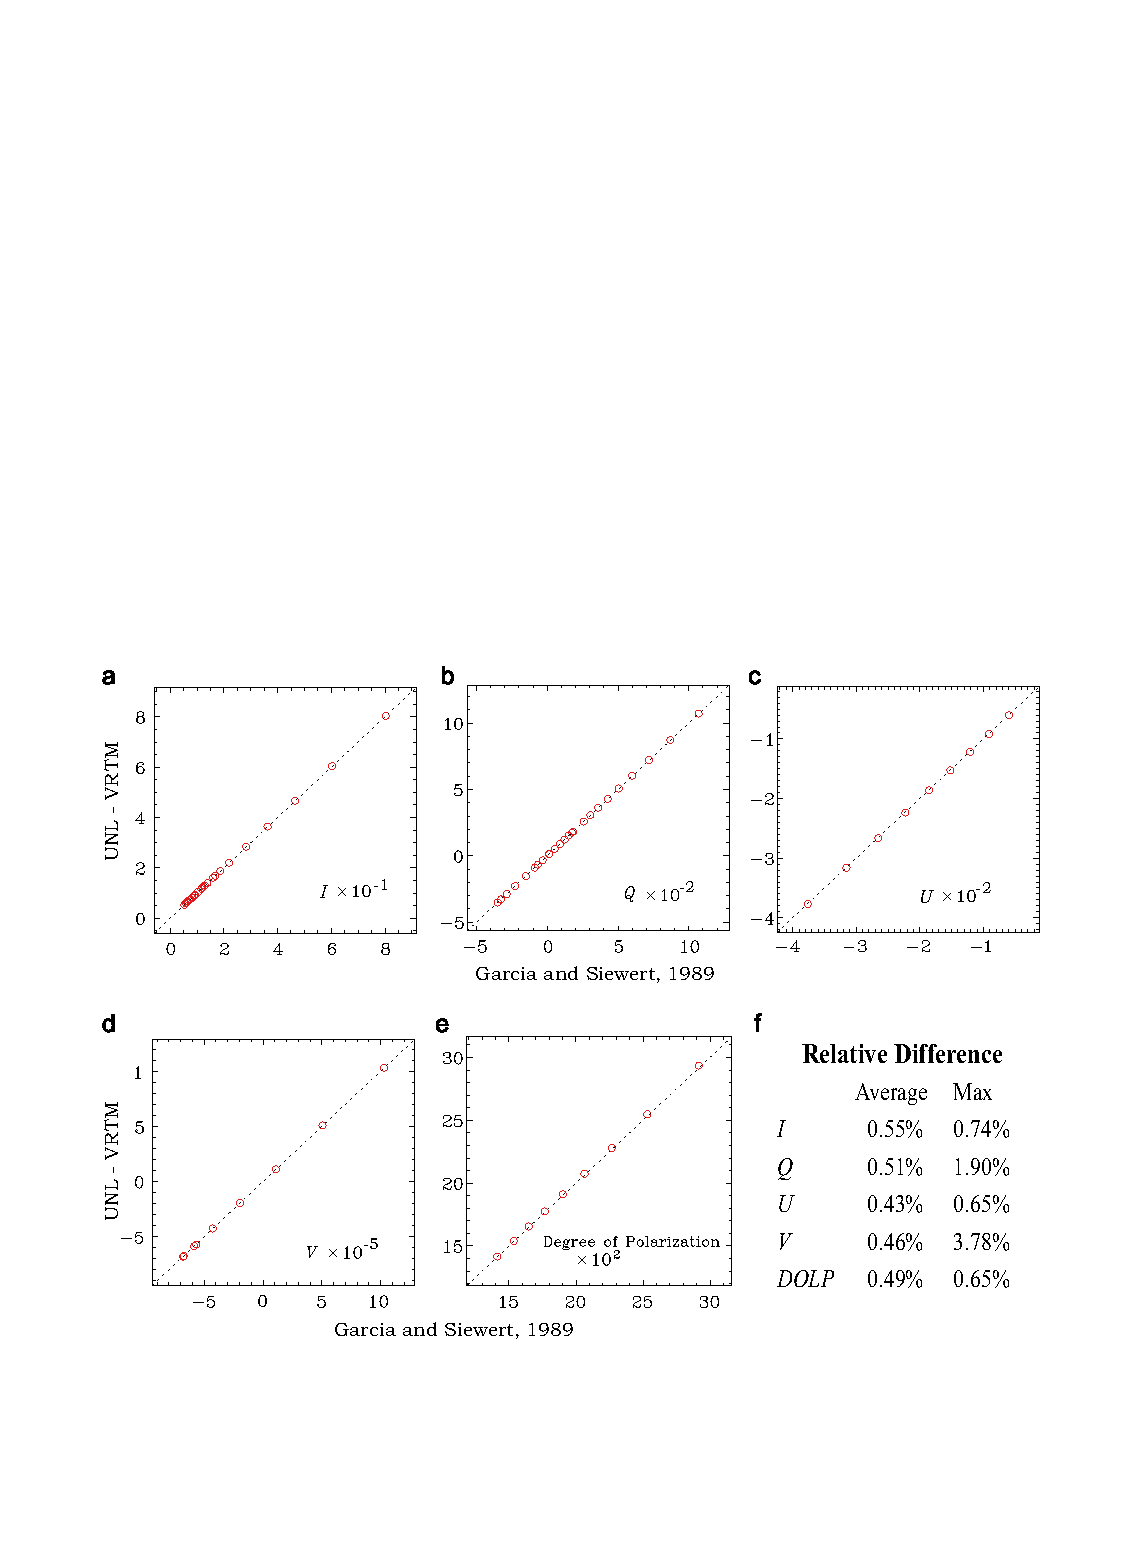
\includegraphics[width={0.8\textwidth}]{figures/unlvrtm3.pdf}
  \caption{Counterparts in Tables 3--10 of \citet{Garcia89} for
upwelling radiation on the top of the same atmospheric conditions of
aerosol scattering. No gas absorption and Rayleigh scattering are
considered. Note that compared here are $I$ and $Q$ values reported 
in \citet{Garcia89} for 9 view angles (with cosine values from 0.1 
to 0.9 at equal spacing of 0.1) and 3 relative azimuth angles 
(0, $\pi/2$, and $\pi$), which yields a total of 27 data points. 
For $U$ and $V$, their values are reported for the same 9 viewing angles 
but for one relative azimuth angle ($\pi/2$) only. 
The calculation is performed at wavelength of 951 nm and $\tau$ of 1.0, 
and aerosol size distribution parameters $\reff=0.2$, 
$\veff=0.07$, refractive index $\mreal=1.44$, and SSA of 0.99.
(Figure adopted from \citet{Wang14}.)}
  \label{fig:unlvrtm3}
\end{figure}

Figure \ref{fig:unlvrtm2} shows the calculation of the degree of linear 
polarization (DOLP) of downward radiation in a pure Rayleigh scattering 
atmosphere. The solid blue line in Figure \ref{fig:unlvrtm2}a (dotted 
line in Figure \ref{fig:unlvrtm2}b) reproduces the theoretical results 
shown in Figure 5.7 of \citet{Coulson88}, which was used to interpret 
the DOLP measured at Mauna Loa Observatory on February 19, 1977. 
Furthermore, Figure \ref{fig:unlvrtm2}a shows that the anisotropy in
Rayleigh scattering reduces the peak DOLP by 5\% (e.g., the difference
between the green and red lines) at 0.7 $\mu$m. Surface reflection and its
concomitant increase of atmosphere scattering will decrease the DOLP of
downward radiation. An increase of surface reflectance from 0 to 0.25
decreases the peak DOLP by 10\%.

Quantitatively, the Stokes-vector $I$, $Q$, and $U$ components computed with
UNL-VRTM differ from their counterparts found in the tables by
\citet{Coulson60} by average (relative) deviations of $1.9\times 10^{-4}$
(0.05\%), $2\times 10^{-5}$ (0.14\%), and $4\times 10^{-5}$ (0.03\%), 
respectively (Figure \ref{fig:unlvrtm2}c--e). These
differences are similar to the values $2.1\times 10^{-4}$, $9\times
10^{-5}$, and $4\times 7^{-5}$ identified by \citet{Evans91}. More recently,
Rayleigh-atmosphere benchmark results have been re-computed by
\citet{Vijay12} to a much higher degree of accuracy; this work also
included benchmarking of the VLIDORT model.

Figure \ref{fig:unlvrtm3} shows benchmark calculations of four 
Stokes parameters for radiative transfer in an aerosol-only atmosphere.
\citet{Garcia89} documented their results for unpolarized incident 
radiation at 951 nm and $cos{\Theta_0}$ of 0.2, for an atmosphere with a
Lambertian reflectance of 0.1. The aerosols in that atmosphere were
assumed to satisfy a gamma-function size distribution with $\reff$ of
0.2 $\mu$m and $\veff$ of 0.07, and a refractive index yielding an 
aerosol single scattering albedo of 0.99. Compared to their results, 
the Stokes parameters computed by UNL-VRTM show relative differences 
of less than 0.6\%, with maximum relative differences 
(at certain viewing geometries) of up to 2\% for $Q$ and 3.8\% for $V$. 
The DOLP computed from the UNL-VRTM (with 15 streams for the hemisphere) 
and documented by \citet{Garcia89} (with 3 streams) differ on average 
by 0.5\%, with a maximum relative difference of 0.65\%.

The simultaneous calculation of analytic Jacobians of the four Stokes
parameters with respect to the aerosol optical depth, size parameters,
refractive indices, and aerosol-loading peak height for both fine and
coarse model aerosols may be validated against Jacobians calculated
using the finite difference method (Figures \ref{fig:unlvrtm4} and
\ref{fig:unlvrtm5}). Overall, results from the two methods are 
highly correlated as seen in the scatter plots
shown in these figures. Relative differences in all comparisons are
less than 0.5\%, and in many cases the differences are less than 0.05\%.

\begin{landscape}
\begin{figure}[p]
  \centering
  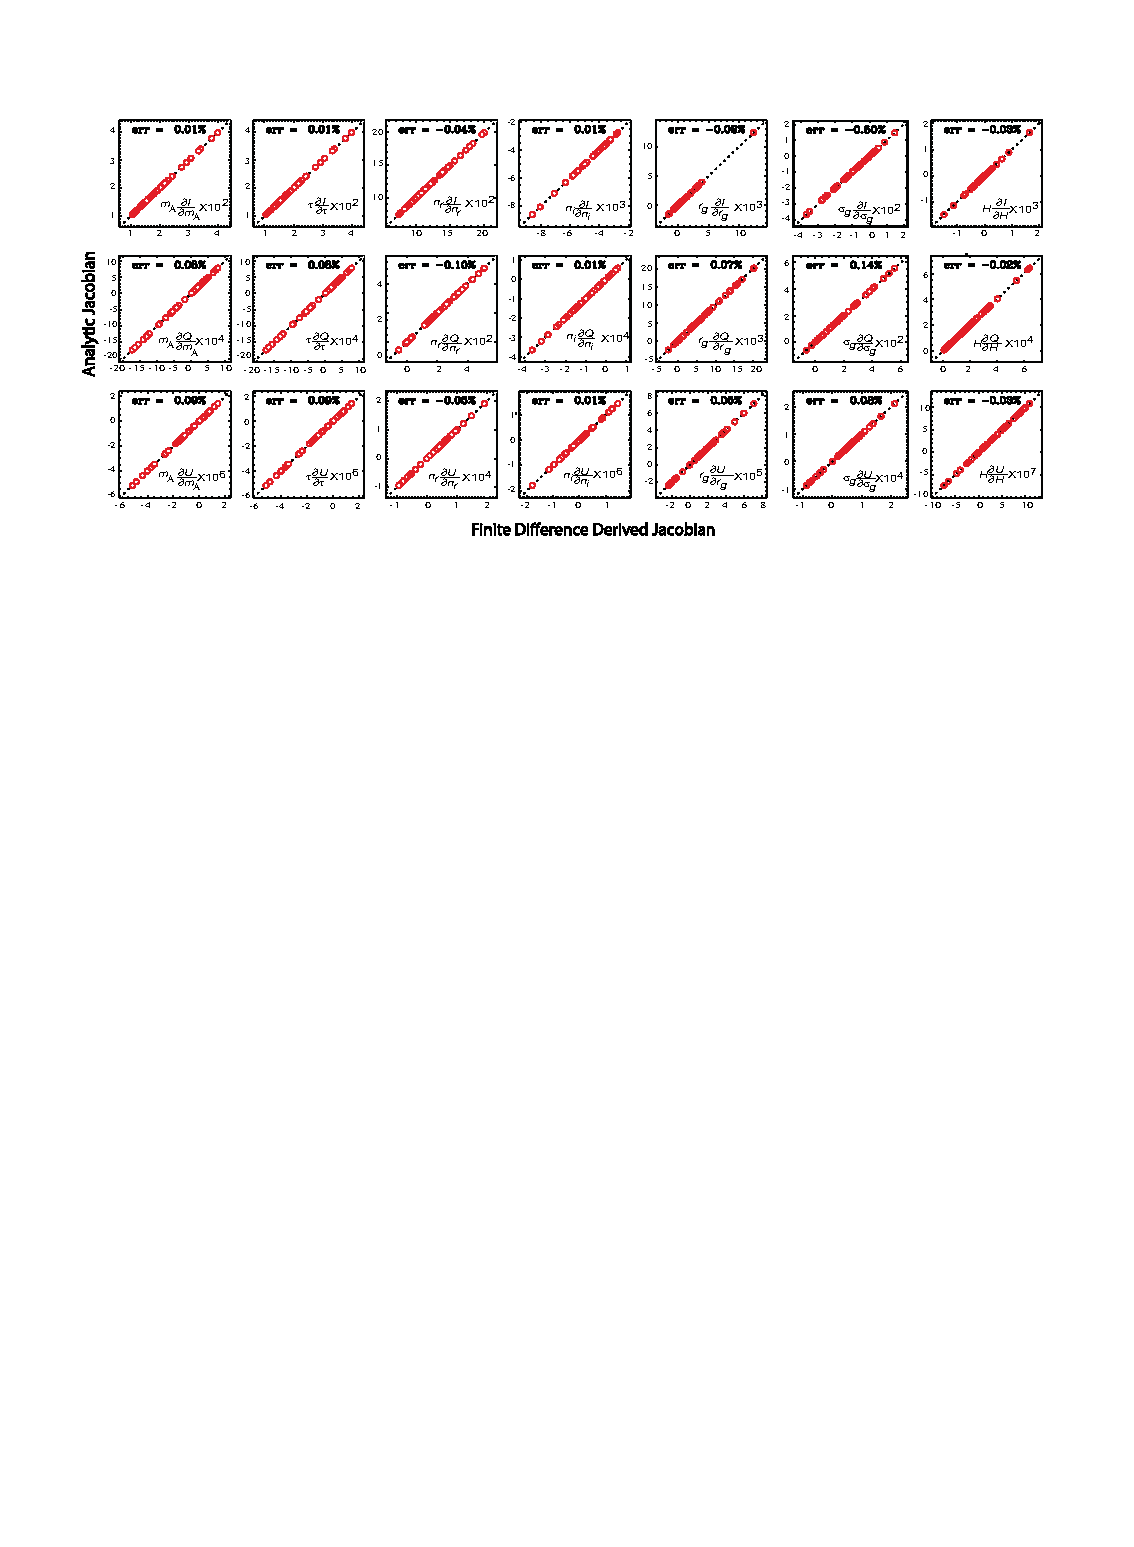
\includegraphics[width={1.4\textwidth}]{figures/unlvrtm4.pdf}
  \caption{Intercomparison of Jacobians ($\ptxi/\partial\ln{x}$) 
calculated with UNL-VRTM using the analytical method (y-axis) with 
those computed from UNL-VRTM using finite-difference estimates (x-axis). 
Here $\xi$ is one of the Stokes parameters: $I$ (top row), $Q$
(middle row), and $U$ (last row). x is one of 7 parameters associated 
with fine-mode aerosols: mass concentration $m_\text{A}$, $\taua$,
$\mreal$, $\mimag$, $\rg$ and $\sg$ (of the lognormal PSD), and height
($H$) of peak aerosol concentration in the vertical. Note,
the calculation is done for an atmosphere containing both fine- 
and coarse-mode aerosols as described in \citet{Hess98}.
(Figure adopted from \citet{Wang14}.)}
  \label{fig:unlvrtm4}
\end{figure}
\end{landscape}

\begin{landscape}
\begin{figure}[p]
  \centering
  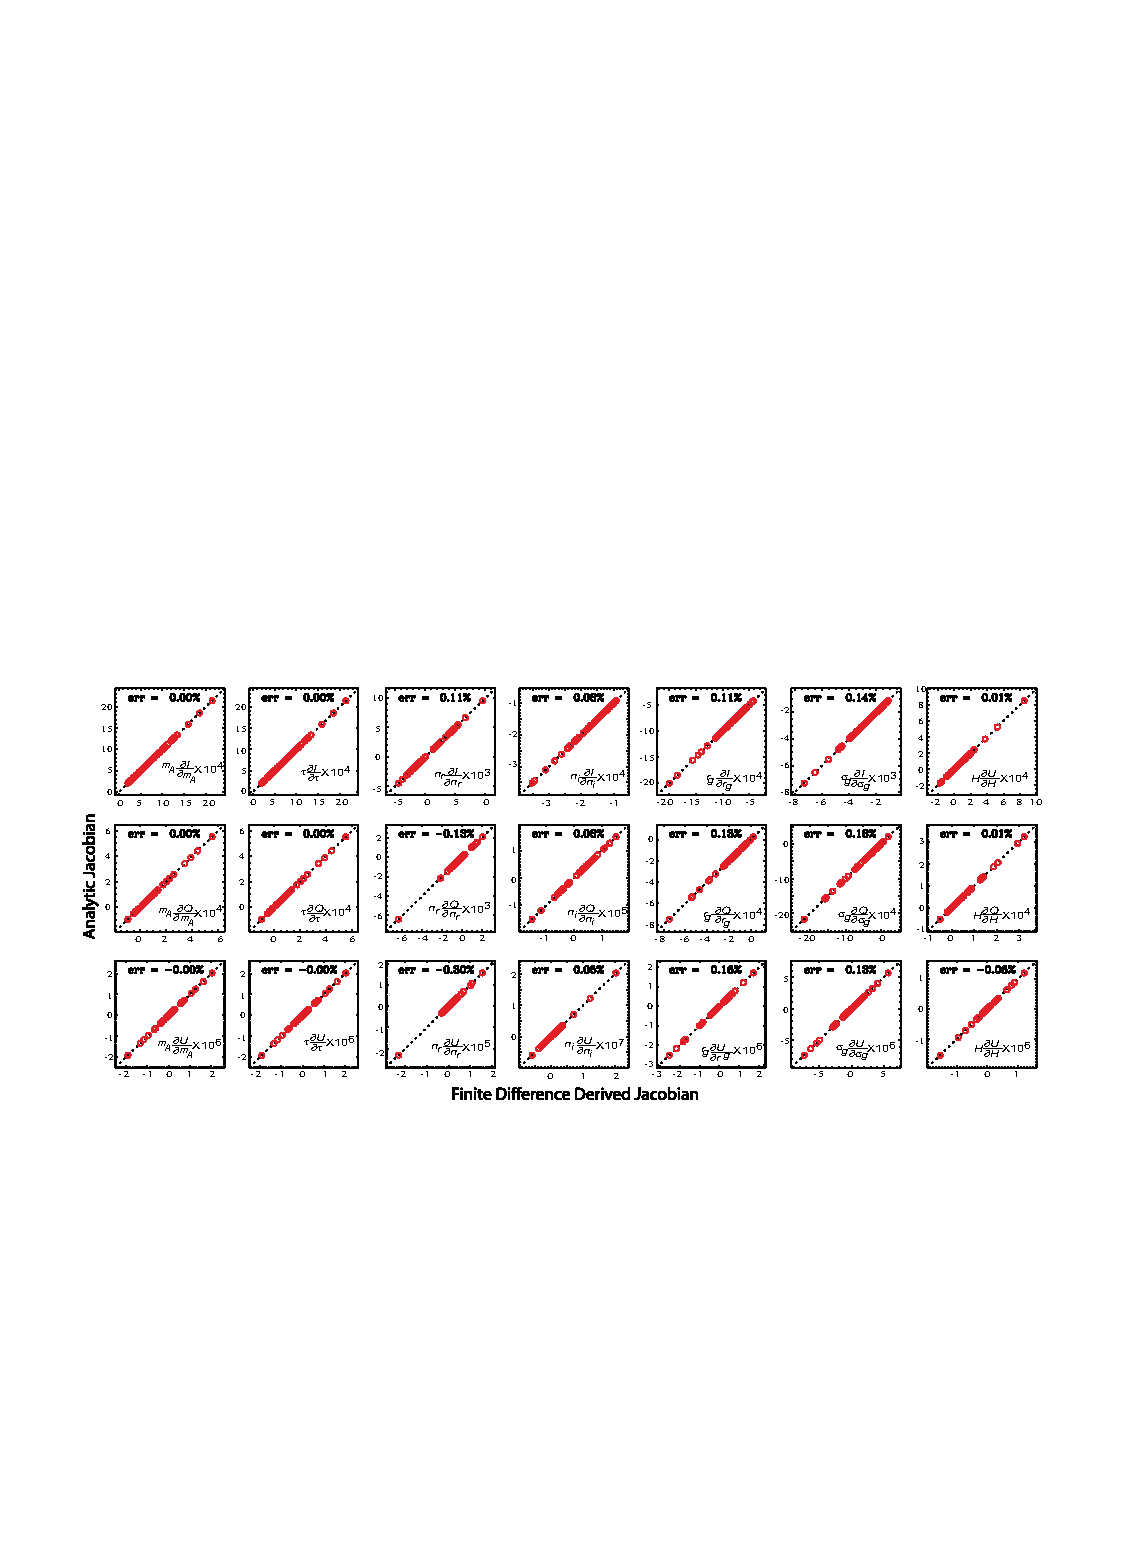
\includegraphics[width={1.4\textwidth}]{figures/unlvrtm5.pdf}
  \caption{Same as in Fig. 5, but for coarse mode aerosols.
(Figure adopted from \citet{Wang14}) }
  \label{fig:unlvrtm5}
\end{figure}
\end{landscape}
